\chapter{Attribution-based Personas}
\label{Personas}

As explained in Introduction \ref{Introduction}, a case study can help retrieve descriptive and explanatory insights regarding a phenomenon, alongside the more common, exploratory ones. After conducting interviews and a survey with the participants of this research, the gathered data presented the opportunity to indeed augment the investigated behaviours and biases with more explanations, justifications and reasonings. These would be directly obtained from the open questions of the interviews and the survey itself.

To better structure such information, we opted for the development of \textit{personas}. Alan Cooper, who conceptualized them, explained that "personas are not real people, but they are based on the behaviors and motivations of real people we have observed and represent them throughout the design process" \cite{Cooper2007}. The design process Cooper describes, relates to the early phases of the development of any product, be this software-based or a tangible product.

The process of persona development also overlaps with the one followed in our research. Its first phase is focused on research, and it emphasizes the retrieval of qualitative data. It usually includes observations and one-on-one interviews with the stakeholders. According to Cooper, one of the principal outcomes of observation and interviews is an emergent set of behavior patterns, which are identifiable behaviors that help categorize modes of use of a potential or existing product. These patterns furthermore suggest goals and motivations \cite{Cooper2007}.

Although we will not be using the concept of personas to represent users of a product or service, the notions and processes are beneficial to build a more complete and comprehensible portrayal of attribution biases. There will be no "mode of use", but rather modes of operation of people exhibiting certain behaviours, all from the perspective and perceptions of the project leaders. 

The first section of this chapter will describe the motivation and process of identifying personas. In \nameref{DefiningAPersona}, we will elaborate more on what constitutes a persona. Lastly, the third section of this chapter will then present the personas that have been developed with their most identifiable characteristics.

\section{Connecting Behaviours - Attributions - Personas}

The process of constructing personas was directly related to answering RQ2: \textit{Can similarities between perceptions be identified and structured in the form of personas?} and made use of the data set gathered from the interviews and the survey. 

As described in \nameref{questionnaireDesignProcess}, the responses of the questionnaire were derived from the attributions identified in the semi-structured interviews, therefore, the process of linking attributions to behaviours was initially undertaken during the creation of the survey questionnaire itself. To recapitalize, the answers of the interview questions were analysed to derive the most dominant attributions PLs would make on certain behaviours. 

Considering personas to be compilations of attributions, the set of responses served as a basis with which initial clusters could be built. The process of clustering attributions followed the logic of thematic analysis, in which a combination of semantic and syntactic analysis methods was employed. Subject of the thematic analysis were initially the questionnaire closed question responses. These would iteratively be completed by the open questions' answers.

In the first round of clustering, which relied primarily on syntactical analysis, a set of 10 clusters was identified. The words that would be repeated the most often were \textit{unprofessional, rude, uninterested, disrespectful, unmotivated} and \textit{distracted}. These were present not only in the survey responses, but in the interviews as well. 

Having identified these clusters, the iterations to come focused on identifying subpatterns and attempting to merge the clusters furthermore. Emphasis was laid on the intention of the statements, perception over personality of the potential persona and various similarities, which would change from persona to persona.

The final round of persona creation based on the survey responses can be found in \nameref{Appendix}. At the end, we settled for a set of 5 major personas (\textit{The Unprofessional, Ego is the enemy, L'Étranger, The Loner, Ther Unterperformer}), with their own subpatterns, and 2 minor personas (\textit{Hiding and not Seeking, Distraction Monster}). What and how we decided to present the information regarding a persona, will be explained in the following section.

\section{Defining a persona} \label{DefiningAPersona}

The personas are designed to have (at least) one main distinctive trait, which ought to be represented in the name of each persona as well. Each persona needs to be equipped with a description, elaborating these distinctive features, and setting up the expectations for this persona in terms of attributions and behaviours. In typical persona representation, the personas are accompanied by an image.

The more important content of a persona, would include a list of attributions that are associated with this persona and the behaviours triggering such an attribution. The list of attributions on a persona display the exact goal of this phase of the thesis. Not only did we intent to identify patterns within perceptions, that would consequently define personas, but we also wanted to provide each persona with a set of perceptions that would point to this same pattern.

As a behaviour can be perceived differently from different PLs and be associated with multiple attributions, the same can be observed for attributions as well. The similar attributions can be made for different behaviours, and this has been noticed especially within the same person/interview. Therefore, as a characteristic of a persona, we want to provide behaviours which entice the attribution as well. As described in the introduction of this chapter, by adding behaviours we want to present the way these personas interact with the remote setting and remote team.

Considering that the data originates from interviews \textit{and} surveys, open \textit{and} closed questions, we have divided the information regarding attributions and behaviours in two categories, to increase readability and transparency regarding the retrieval of the data. More about the constructing technicality of these two aspects, can be found in the next chapter.


\section{Personas} \label{Personas}

In this section we will be presenting the personas we were able to develop. The data regarding a persona will be presented in a tabular form, as this is the typical representation of a persona. Each persona has a title, to identify personas but also to already indicate about their distinct characteristics. A description will follow, which is derived from the understanding PLs have of the main attributions. To add a more human touch to the personas, they are also enhanced with a representative image. Next, a list of attributions will follow which we believe to be associated with the description and title of the persona. 

Considering that the data has been collected either via closed questions (CQ) or open questions (OQ), we make this distinction in the presentation of attributions and behaviours too. Each CQ attribution is followed by the question of the survey, which includes the attribution as a response statement, and the frenquency with which the respondents have answered with Agree or Strongly Agree. The OQ attributions can be followed by the question code too, indicating that this is an attribution made in regards to the question and the behaviour associated with that question. If the OQ attribution is followed by the interview code, that is an indicator that the statement has been retrieved from a specific interview. 

Behaviours are divided similarly, where the code is stated at the beginning of each entry in the CQ column. The CQ Behaviours are too followed by the agreement percentage of the statement that relates to that persona. This percentage can be read the following way: If Q3 has 87,5\% in persona X, it means that 87,5\% of respondents (at least) agree that the behaviour exhibited in Q3 relates to persona X. The CQ Behaviours column is in descending order. 

The last section of the table presents suggestions made by PLs on how to deal with some of the personas, based on the attributions and typical behaviours. These are retrieved primarily from the semi-structured interviews. 

\subsection{The Unprofessional}

The term "unprofessional" was associated with 5 of the survey responses and it was mentioned 3 times in the open questions of the survey. This group of attribution is one of the biggest we have identified, and an important one. What was considered unprofessional, was behaviour that didn't conform to the expectations of a specific situation or the participants of a meeting. Generally, unprofessionalism was considered unintentional and was linked to immaturity, considering the later one also unintentional. 

\begin{longtable}[ht]{ p{0.15\textwidth}  p{0.4\textwidth} p{0.4\textwidth} }
\caption{The Unprofessional Persona}
\label{tab:theUnprofessional}\\
\hline
\textbf{Title} & The Unprofessional \\
    \hline
   \textbf{Description } & \multicolumn{2}{p{.80\textwidth}}{Attribution based on behaviour that does not conform to the one expected by the team. Usually considered unintentional.}  \\
   \hline
   \textbf{Image} &  
\includegraphics[valign=t, width=1in, margin=0pt 3pt 0pt 3pt]{figures/TheUnprofessional.png} \\
    \hline
    & \textbf{Closed Questions} & \textbf{Open Questions} \\
    \hline
    \multirow{5}{3cm}{\textbf{Behaviours}}  & Q8: Constantly interacting with the mobile phone. Typical behaviours include checking notifications, taking phone calls while in the meeting, obviously typing on the device (100\%) &  Directly contacting the customers (I1) \\
     &  Q14: Engaging in physical activity, like walking around or performing some physical exercise (88,9\%) & Disagreeing to using a certain tool (I3) \\
     & Q1: Joins meetings from their phone while engaging in an other activity like running errands, commuting (88,9\%) & Generally when unnecessary things happen behind their backs and are shown in the camera (I7) \\
 	 & Q12: Having audio issues and very bad quality of sound (55,6\%) & it is even worse when the sound is too loud (Q12)  \\
 & Q5: A person enters/is in the room of one of the participants and they might even engage in conversation (33,3\%) & This behaviour is considered especially unprofessional when there is communication with the other person in the room (Q5) \\
    \hline
    \multirow{6}{3cm}{\textbf{Attributions}}  & I would personally consider this quite unprofessional (A1.4,  66,6\%) & This unprofessionalism translates into their work (I1) \\
     & They probably easily mix private and professional life (A5.4,  33,3\%) &  If unprofessional behaviour is intentional, I would consider it even rude (I3) \\
     & This is quite an immature thing to do in meetings (A8.2, 100\%) & They do not care about being perceived as unprofessional. But some people might be offended (I7) \\
 	 & They should consider switching or investing in a more professional setting (A12.1, 55,6\%) \\
 	 & To me,  it shows an unwillingness to adapt to a professional setting (A14.2, 88,9\%) \\
 	\hline
    \textbf{Suggested Reactions} & \multicolumn{2}{p{.80\textwidth}}{This persona might exhibit inappropriate behaviour in more serious situations. Therefore, the project leader can opt to talk about it to everyone in the internal team meetings, or if there is time-sensitivity, directly contact the person.} \\
    \hline
\label{tab:multicol}
\end{longtable}

\subsection{Ego is the enemy}

This persona is a constellation of traits that refer to putting oneself at the certain of a situation, often intentionally. The sense of being egoistical is intertwined with being oblivious to the fact the person is part of the team. The displayed behaviours are often perceived as being disrespectful towards the other participants of the meeting. 

\begin{longtable}[ht]{ p{0.15\textwidth}  p{0.4\textwidth} p{0.4\textwidth} }
\caption{Ego is the enemy Persona}
\label{tab:theEgo}\\
\hline
\textbf{Title} & Ego is the enemy \\
    \hline
   \textbf{Description} & \multicolumn{2}{p{.80\textwidth}}{Attribution formed based on egoistical attitude and behaviour of a person, which often overshadows the efforts of the other members and might even be offensive in more serious cases.}  \\
   \hline
   \textbf{Image} &  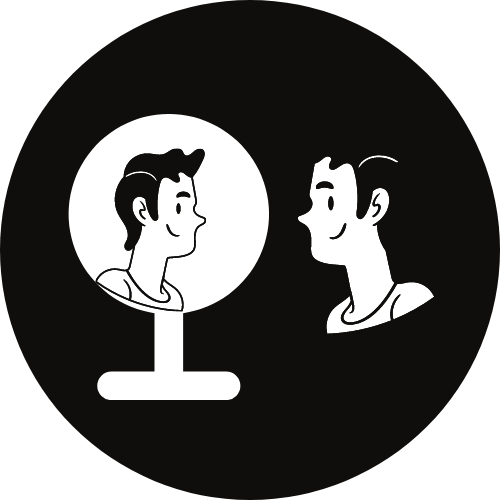
\includegraphics[valign=t, width=1in, margin=0pt 3pt 0pt 3pt]{figures/Ego.png} \\
    \hline
    & \textbf{Closed Questions} & \textbf{Open Questions} \\
    \hline
    \multirow{5}{3cm}{\textbf{Behaviours}}  & Q3: Constantly interacting with the mobile phone by looking at it, checking notifications, taking phone calls, even type… (100\%) & Not giving the other team members complex tasks (I2) \\
     &  Q4: One of the team members constantly turns their camera on and off to do something meanwhile (87,5\%). & Of course there is rude behaviour, like exit the zoom meeting without saying anything (I3) \\
     & Q13: A student constantly interrupts/talks over the participants of a meeting (62,5\%). &  Coming late to the meeting or leaving early quite often (I3) \\
 	 & Q14: Engaging in physical activity, like walking around or performing some physical exercise(75\%)  \\
 	 & Q5: A person enters/is in the room of one of the participants and they might even engage in conversation (62,5\%) \\
 	\hline
    \multirow{6}{3cm}{\textbf{Attributions}}  & I would consider this impolite towards the participants of the meeting (A3.1, 100\%) & They were disrespectful not only towards me, but also towards themselves (I2) \\
     & It’s confusing to me why they do this and a bit disrespectful (A4.2, 87,5\%)&  Undermining the female participant as a sign of toxic masculinity (I2) \\
     & This might be offensive towards the participants in the meeting (A5.1, 62,5\%) & Disrespectful towards the contribution others are giving to the meeting (I7) \\
     & This could be disrespectful to the participants, especially in formal meetings (A9.2, 25\%)  \\
 	 & They want to impose their opinion on others (A13.1, 87,5\%)   \\
 	 & That don't want the other members to be heard which is quite improper (A13.2, 37,5\%)\\
 	 & This is personally even rude (A13.3, 62,5\%) \\
 	 & This is inconsiderate towards the other participants (A14.1, 75\%) \\
    \hline 
 	 \textbf{Suggested Reactions} & \multicolumn{2}{p{.80\textwidth}}{This is a difficult situation. PLs emphasize addressing the issue as soon as possible, as the team members might be affected. They also mention that the remote setting escalates nerve-wrecking situations quickly, therefore, it is crucial to be alert towards the behaviours described in this persona.} \\
    \hline
\label{tab:multicol}
\end{longtable}

\subsection{L'Étranger}

This group of attributions involves perceptions made on individuals not exhibiting any particular interest, priorization or appreciation of the project. According to PLs, this is shown in the form of non-participation, or sporadic, irrelevant engagement. Considering the answers given by the PLs, this persona was constructed with attributions pointing at a low conscientiousness of the individual. The name of this persona relates to the main character in Albert Camus' \textit{L'Étranger}, who was completely detached from the happenings around his existence. 

\begin{longtable}[ht]{ p{0.15\textwidth}  p{0.4\textwidth} p{0.4\textwidth} }
\caption{L'Étranger Persona}
\label{tab:theDetached}\\
\hline
\textbf{Title} & L'Étranger \\
    \hline
   \textbf{Description} &  \multicolumn{2}{p{.80\textwidth}}{This Persona represents a person detached and disengaged from the activities of a meeting. They are usually not as involved as other participants and therefore, stand out for their distance.} \\
   \hline
   \textbf{Image} &  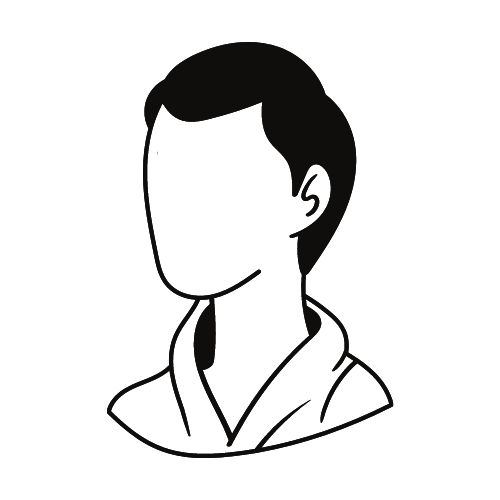
\includegraphics[valign=t, width=1in, margin=0pt 3pt 0pt 3pt]{figures/TheStranger.png} \\
   \hline
    & \textbf{Closed Questions} & \textbf{Open Questions} \\
    \hline
    \multirow{4}{3cm}{\textbf{Behaviours}}  & Q8: Constantly interacting with the mobile phone. Typical behaviours include checking notifications, taking phone calls while in the meeting, obviously typing on the device (100\%) & Having the camera off (I1) \\
     &  Q1: Joins meetings from their phone while engaging in an other activity like running errands, commuting (87,5\%).  & Apologizing without giving any valid reason or excuse for being late of joining from other places  (I2) \\
     & Q3: A person is actively doing something besides the meeting on their computer (seems focused on another task, are typing) (75\%). & Giving the impression the team member is not aware about what is happening (I3) \\
 	 & Q7: A person in the team is slouching and looking quite sleepy… (37,5\%) & Not sharing their opinion on important issues or just passively agreeing (I4) \\
    \hline
    \multirow{10}{3cm}{\textbf{Attributions}}  & They are actually not attentive and must schedule more time for the meetings (A1.1, 87,5\%) & I get the feeling I am interacting with a clam (I1)  \\
     & This person isn't particularly interested in getting the most out of the iPraktikum and the meeting (A1.3, 87,5\%) & They consciously make a decision to not care about what the others are saying (I4) \\
     & They consider the iPraktikum the typical uni lecture and are just there to not absent (A2.4, 25\%) & It seems to me that they are bored (I7) \\
     & The advancement of the project might not be a priority (A3.2, 75\%) \\
     & The project itself is seemingly not appealing to them (A3.3, 33,3\%) \\
 	 & They might not be really interested in the project and are just pretending to agree (A6.3, 25\%)  \\
 	 & They might consider it unnecessary to get out of the comfort zone of their home and make an extra effort (A7.3, 37,5\%) \\
 	 & They are not interested in the discussion and in what everyone else is saying (A8.3, 100\%) \\
 	 & The iPraktikum is not a priority to them this semester (A11.1, 25\%) \\
 	 & They are probably just opening the page before having to share the screen (A11.2,  22,2\%) \\
    \hline   
     \textbf{Suggested Reactions} & \multicolumn{2}{p{.80\textwidth}}{In case of disinterest, there is often not much one can do, as no one can force another person to like or engage in anything. As a few PLs have mentioned, participants in the iPraktikum are adults, and can make their own decisions.} \\
    \hline
\label{tab:multicol}
\end{longtable}

\subsection{The Loner}

The difference from the detached persona is that with this persona we do not imply a lack of interest. There might other perceptions explaining the distance between the person and the other participants, and assumptions regarding the relationship and collaboration with the team. The most common perceptions are that the person in introverted, not being a team member and generally being insecure or unmotivated. Lacking motivation is included in this persona, as it is linked with introversion and a person being more isolated. 

\begin{longtable}[ht]{ p{0.15\textwidth}  p{0.4\textwidth} p{0.4\textwidth} }
\caption{The Loner Persona}
\label{tab:theLoner}\\
\hline
\textbf{Title} & The Loner \\
    \hline
   \textbf{Description} & \multicolumn{2}{p{.80\textwidth}}{A loner is a person that seems to be operating in a more solitary manner and rises therefore questions regarding their engagement, involvement and personality.} \\
\hline
   \textbf{Image} &  
\includegraphics[valign=t, width=1in, margin=0pt 3pt 0pt 3pt]{figures/Loner.png} \\   
   \hline
    & \textbf{Closed Questions} & \textbf{Open Questions} \\
    \hline
    \multirow{4}{4cm}{\textbf{Behaviours}}  & Q12: AHaving audio issues and very bad quality of sound (100\%) & A person sits in the dark and you can barely see their face (I9) \\
     & Q2: A person in your team is mostly just listening during the meetings and is muted almost all the time (87,5\%). \\
     & Q1: Joins meetings from their phone while engaging in an other activity like running errands, commuting (62,5\%). \\
 	 & Q6: A student is agreeing to “too many” things in the meeting or use empty phrases, but are not actually delivering: (62,5\%)  \\
    \hline
    \multirow{6}{4cm}{\textbf{Attributions}}  & This person might not be involved in the team spirit (A1.2, 62,5\%) & The person may think their work / opinion is not that important. (Q2)  \\
     & They are just shy/introverted (A2.3, 87,5\%) & They might be afraid to express their own opinion and doubts. (Q6) \\
     & Not getting enough feedback makes me think this is not a person you can easily deal with (A6.2, 25\%) & Attributing a behaviour to "nerdness" (Q10) \\
     & It’s not in their culture/personality to reply or ask for support  (A6.4, 62,5)\%\\
 	 & They might not be the most engaged and cooperative in the team (A10.3, 25\%) \\
 	 & It might hurt the quality of the meeting and it renders the person less approachable (A12.2, 100\%)\\
 	 & It makes me think that this person is not motivated (A12.3, 11,1\%) \\
    \hline
     \textbf{Suggested Reactions} & \multicolumn{2}{p{.80\textwidth}}{PLs have mentioned often being mistaken about the people not being as dominant as others. Therefore, it is important here to keep an eye on the progress of the tasks, and the perceptions the other team members have on this person. Ice-breakers are also perceived as the traditional remedy to bringing teams together.} \\
    \hline
\label{tab:multicol}
\end{longtable}

\subsection{The Underperformer}

The perception created on this persona is generally that they are not performing on the same level as the other participants of the team. PLs in this case, try to reason why this is the case. Typical attributions can relate directly to poor performance or indirectly to avoiding work, lack of experience, etc.

\begin{longtable}[ht]{ p{0.15\textwidth}  p{0.4\textwidth} p{0.4\textwidth} }
\caption{The Underperformer Persona}
\label{tab:underperformer}\\
\hline
\textbf{Title} & The Underperformer \\
    \hline
   \textbf{Description} &  \multicolumn{2}{p{.80\textwidth}}{Attributions related to this persona are usually made with the goal of explaining this person's lack of performance or a tendency to perform in a poorer manner.} \\
   \hline
   \textbf{Image} &  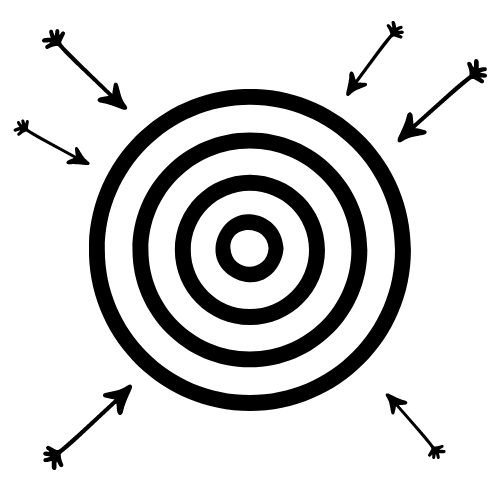
\includegraphics[valign=t, width=1in, margin=0pt 3pt 0pt 3pt]{figures/OffTarget.png} \\
   \hline
    & \textbf{Closed Questions} & \textbf{Open Questions} \\
    \hline
    \multirow{5}{4cm}{\textbf{Behaviours}}  & Q3: But then you realize that a person is actively doing something besides the meeting on their computer (seems focused on another task, are typing) (37,5\%)  & Not trying to improve the situation regarding their tech setup (I4) \\
     & Q4: One of the team members constantly turns their camera on and off to do something meanwhile (37,5\%) & Being too optimistic and asking about the consequences of not achieving something on time (I3) \\
     & Q2: A person in your team is mostly just listening during the meetings and is muted almost all the time (25\%) &  Giving the impression one is not fully grasping what needs to be done (I1) \\
 	 & Q7: A person in the team is slouching and looking quite sleepy…(25\%)  \\
 	 & Q9: A student has a stack of dishes waiting to be cleaned or a pile of clothes behind. (25\%)  \\
    \hline
    \multirow{7}{4cm}{\textbf{Attributions}}  & They probably just want to pretend to be in the meeting, but not put in the work (A3.4, 37,5\%) & Thinking a person is lazy (I1, I3) \\
     & This could make me suspicious of their performance (A10.2, 12,5\%) \\
     & I would assume they are not that committed to the project and teamwork (A4.1, 37,5\%) \\
     & They are likely facing impediments with their tasks/ struggling with productivity (A2.5, 25\%) \\
     & This "sluggishness" probably translates into their work (A7.2, 25\%) \\
 	 & This person might be disorganized in their work too (A9.1, 25\%) \\
 	 & This person is probably not as experienced as the others  (A2.1, 11,1\%) \\
 	 & They might be lacking the skills to keep up to their promises (A6.1, 100\%) \\    
    \hline
     \textbf{Suggested Reactions} & \multicolumn{2}{p{.80\textwidth}}{ If the PL reasons that the person is facing difficulties, it might be beneficial to ask the coach to gather more insights about one's impediments. But as this might just be a perception, tracking the performance through other tools such as Jira and Bitbucket is the more accurate evaluation of one's performance. } \\
    \hline
\label{tab:multicol}
\end{longtable}

\subsection{Hiding and not seeking}

This persona is presumably trying to hide something, whether it is in regards to something personal or related to the project. It is often assumed that this persona is not actively trying to change something about their presence in the meeting.

\begin{longtable}[ht]{ p{0.15\textwidth}  p{0.4\textwidth} p{0.4\textwidth} }
\caption{Hiding and not seeking Persona}
\label{tab:hiding}\\
\hline
\textbf{Title} & Hiding and not seeking \\
    \hline
   \textbf{Description} &  \multicolumn{2}{p{.80\textwidth}}{Attributions regarding this persona are made as the PLs notice a tendency to not openly approach the virtual setting} \\
   \hline
   \textbf{Image} &  
\includegraphics[valign=t, width=1in, margin=0pt 3pt 0pt 3pt]{figures/Mask.png} \\
   \hline
    & \textbf{Closed Questions} & \textbf{Open Questions} \\
    \hline
    \multirow{4}{4cm}{\textbf{Behaviours}}  & Q4: One of the team members constantly turns their camera on and off to do something meanwhile (77,8\%). \\
     & Q2: A person in your team is mostly just listening during the meetings and is muted almost all the time (22,2\%). \\
 	 & Q11: One of the participants is facing problems connecting his devices or seems reluctant to do so. You probably also see other things open on their screen (22,2\%)  \\
 	 & Q10: A person doesn’t make themselves visible in the meeting (not because their camera is off, but because they sit in the dark, the camera is in a weird position) (11,1\%) \\
    \hline
    \multirow{4}{4cm}{\textbf{Attributions}}  & I would assume they are doing something else in parallel (A2.2, 22,2\%) & It's easier for the participants to avoid confrontation when you can immediately leave a meeting (I3) \\
     & They are possibly not actively listening and don’t want to show what they are doing instead  (A4.3, 77,8\%) \\
     & They don’t want to show their facial expressions and reactions (A10.1, 11,1\%) \\
     & They might not be actively sharing so they don't have to show their actual progress (A11.3, 22,2\%)\\
    \hline 
     \textbf{Suggested Reactions} & \multicolumn{2}{p{.80\textwidth}}{Some of the PLs compile rules for the remote meeting, which could minimize the probability of someone engaging less than the others.} \\
    \hline
\label{tab:multicol}
\end{longtable}

\subsection{Distraction monster}

Sometimes attribution are made on the level of focus one has, or as in this case, the lack thereof. Distraction was a big theme in the interviews, and a large part of the behaviours PLs consider inappropriate come as a result of distractions. This persona is a minor one though, because when a distraction happens, the typical reaction or attribution is not to say, that they are distracted, but to make an attribution more fitting to the first personas presented in this thesis. Nonetheless, there are attributions directly related to being distracted. We also include being bored, as it might be an indicator of lack of focus.

\begin{longtable}[t]{ p{0.15\textwidth}  p{0.4\textwidth} p{0.4\textwidth} }
\caption{Distraction Monster Persona}
\label{tab:distraction}\\
\hline
\textbf{Title} & Distraction monster \\
    \hline
   \textbf{Description} &  \multicolumn{2}{p{.80\textwidth}}{Attributions of this persona relate to the lack of focus one might exhibit during team meeting activities} \\
   \hline
   \textbf{Image} &  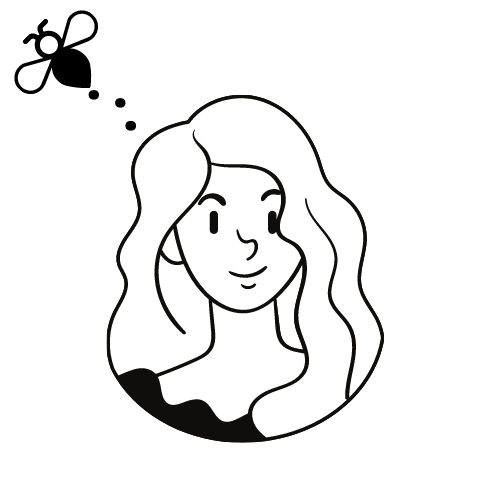
\includegraphics[valign=t, width=1in, margin=0pt 3pt 0pt 3pt]{figures/Distraction.png} \\
   \hline
    & \textbf{Closed Questions} & \textbf{Open Questions} \\
     \hline
    \multirow{4}{4cm}{\textbf{Behaviours}}  & Q8: Constantly interacting with the mobile phone. Typical behaviours include checking notifications, taking phone calls while in the meeting, obviously typing on the device (66,6\%) & Simply looking downwards, or in a direction where a computer screen would not be considered normal (I4) \\
     & Q7: A person in the team is slouching and looking quite sleepy… (55,6\%). \\
     & Q5: A person enters/is in the room of one of the participants and they might even engage in conversation (33,3\%). \\
    \hline
    \multirow{4}{4cm}{\textbf{Attributions}}  & To me, it looks like they are not focused on the meeting and get distracted easily (A5.2, 33,3\%) & It's easier for the participants to avoid confrontation when you can immediately leave a meeting (I3) \\
     & Perhaps, they are bored and are not really attending (A7.1, 55,6\%) \\
     & They could be into social media or communication apps (A8.1, 66,6\%) \\
    \hline
     \textbf{Suggested Reactions} & \multicolumn{2}{p{.80\textwidth}}{What PLs say, it to ask questions to the person that seems distracted, in the hopes of them redirecting their focus into the meeting. } \\
    \hline
\label{tab:multicol}
\end{longtable}

\section{Limitations}

Despite the analogies between the typical personas, and the ones we have developed, the reader must keep in mind that this research's personas are built on perceptions of PLs, and are no factual representations of real people. The focus of personas is \textit{not} the investigation of inappropriate behaviours, or the reasons these behaviours are exhibited. 

The personas presented in this chapter might also resemble antipatterns. Personas personify attribution biases, and, if an antipattern were to be investigated, it would be the one of forming dispositional attributions, rather than the personas in isolation. In order to construct antipatterns, a specific structure must exist, which does not apply to the topic of attribution bias.

Considering the limited resources of this study, it was not feasible to test every behaviour towards every attribution. Considering the dependency from the survey, we can assume that if the survey questionnaire were to be designed differently, the developed personas could differ as well.
